%% content.tex
%%

%% ===========================
\chapter{Konzeption}
%% ===========================

...

%% ===========================
\section{Architektur}
%% ===========================

Nachdem bereits eine Datenbank ausgewählt wurde, kann ein erster Überblick über den groben Aufbau des Systems gegeben werden. In Abbildung \ref{konzept_architektur} können die Zusammenhänge des abzubildenden Software-Systems betrachtet werden. Beim Konzept handelt es sich um Zweischichtenarchitektur, auch bekannt als Client-Server-Architektur.   

\begin{figure}[htbp]
\centering
  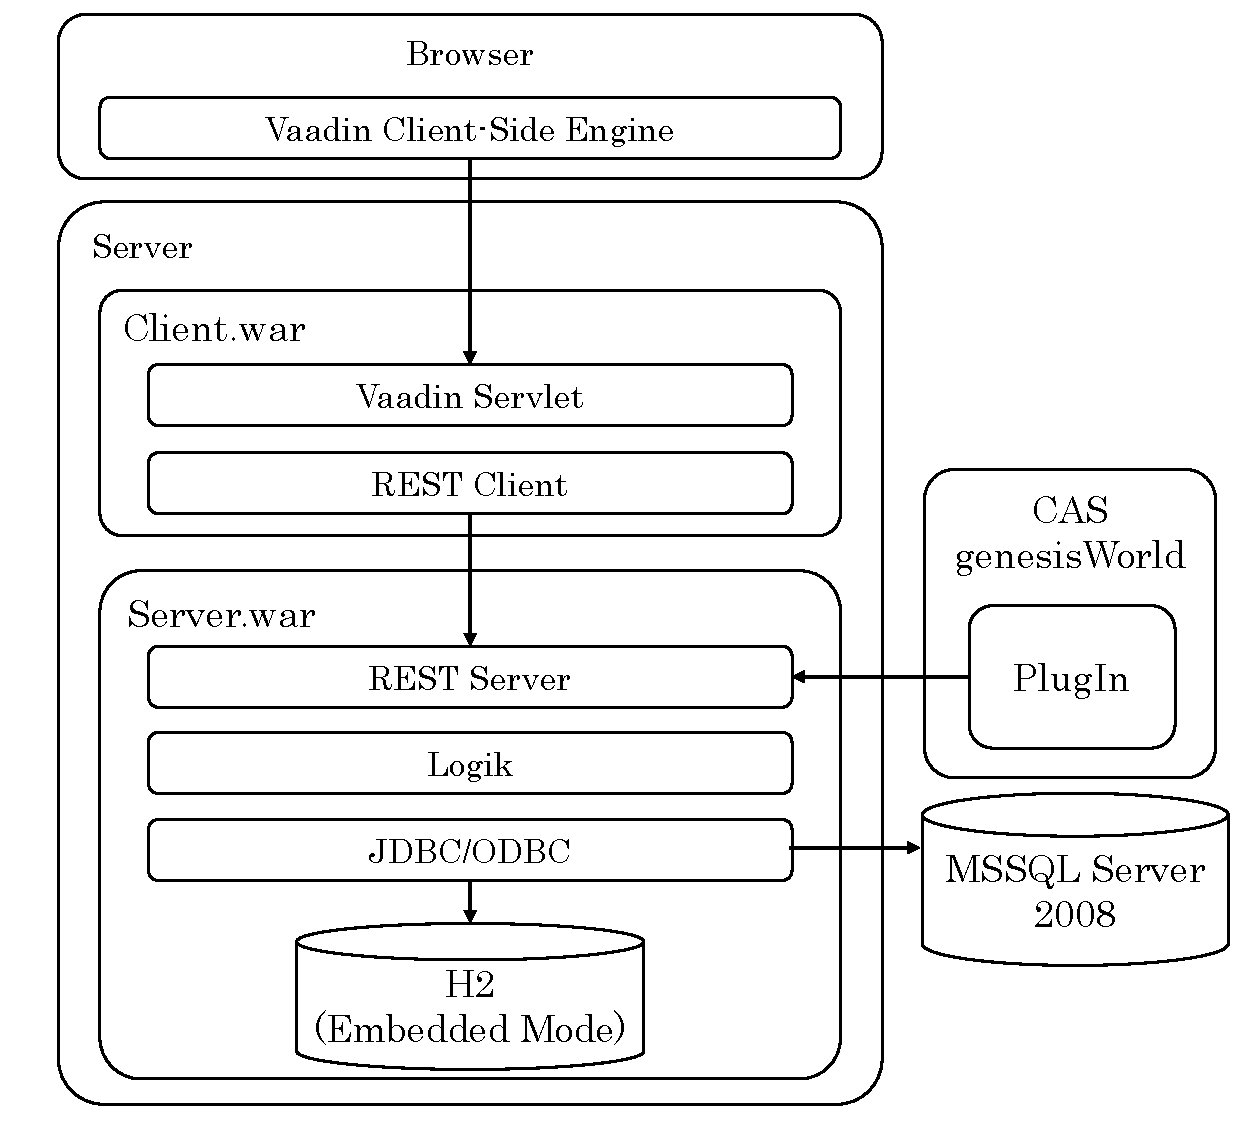
\includegraphics[width=0.8\textwidth, width=0.8\textwidth]{pics/Konzept_architektur.pdf}
\caption{Architektur des Systems}
\label{konzept_architektur}
\end{figure} 

Die Vaadin Client-Side Engine verwaltet das Rendering der Oberfläche im Web-Browser durch den Einsatz verschiedener Client-Seitiger Widgets, die das Gegenstücke zu den serverseitigen Komponenten bilden. Es leitet Benutzerinteraktion an die Server-Seite weiter und rendert anschließend die Änderungen für die Benutzeroberfläche. Die Kommunikation findet über asynchrone HTTP-oder HTTPS-Anfragen statt.

Auf der Server-Seite arbeitet die Vaadin-Anwendungen auf der Java-Servlet-API. Das Vaadin Servlet oder genauer die VaadinServlet Klasse ist für die Delegation verschiedenen Clients zuständig. Sie empfängt Anfragen und legt mithilfe von Cookies fest welche Benutzersitzung zu welchem Client gehört.

Interaktion mit dem Benutzer-Interface-Komponenten erzeugen Events, die zunächst auf der Client-Seite durch die Widgets verarbeitet werden. Nachfolgend werden die Events durch den HTTP-Server, das Vaadin Servlet und durch die Komponenten der Benutzeroberfläche geleitet bis Sie zu den in der Anwendung definierten Event-Listenern gelangen. In den Listenern wird mithilfe des REST-Clients ein POST-Requests an die Logik gesendet. Dieser enthält alle durch den Benutzer eingegeben Werte. 

Der erste Schritt zur Umsetzung der geforderten losen Kopplung zwischen Darstellung und Logik wird durch die Aufsplittung in zwei verschiedene Anwendungen erreicht. Die Client.war beinhaltet die Klassen und Objekte der Darstellung. Wohingegen die Server.war alle Elemente zur Umsetzung der Logik beinhaltet. Die Verwendung des REST-Protokolls zwischen der Client.war und Server.war stellt den nächsten Schritt der losen Kopplung dar. Einer der Vorteile ist das die Funktionen des Systems durch andere Clients abgegriffen werden können ohne Änderungen an bestehendem durchführen zu müssen. Beide war-Dateien werden in einem Apache Tomcat Webserver deployed und können über URLs aufgerufen werden.

Die Logikkomponente in der Architektur stellt eine Zusammenfassung aller Funktionen des Anwendungskerns dar. Sie kümmert sich um die Generierung der Abfragen an die Datenbank. Die Generierung der Abfragen erfolgt dynamisch, damit keine unnötigen Bedingungen die Abfragegeschwindigkeit verringern. Abfragen werden mithilfe der Java Database Connectivity(JDBC) an die Datenbank übermittelt. Neben der Generierung der Abfragen enthält die Logikkomponente Funktionen zum Extrahieren und Transformieren der Daten aus der alten Datenbank. 

Um nicht periodisch Extraktion und Transformation wiederholen zu müssen wird ein selbstgeschriebenes PlugIn im CAS genesisWorld Anwendungsserver eingesetzt. Die Grundidee des PlugIns, ist Benachrichtigungen über Änderungen an das neue System zu übermitteln.

%% ===========================
\section{Technologien}
%% ===========================

Als einer der am meist verbreitetsten Programmiersprachen stellt Java die Grundlage aller verwendeten Technologien dar. Zur Darstellung der Inhalte für den Client wird Vaadin verwendet. Der Apache Tomcat7 nimmt die Rolle des Anwendungsservers ein. Die Kommunikation auf Basis von RESTful Web Services wird mithilfe von Jersey realisiert. OpenSCV wird für das Lesen und Schreiben von CSV-Dateien verwendet. JDBC wird zur Kommunikation zwischen Anwendungsserver und der Datenbank verwendet. Die H2-Datenbank stellt die Datenquelle des Systems dar. Im folgenden werden alle Bestandteile bis auf den H2 der bereits erläutert wurde, etwas näher beschrieben. 

\paragraph{Vaadin}

Vaadin ist ein Open-Source-Java-basiertes Framework für den Aufbau von modernen Web-Anwendungen. Der Kerngedanke des Frameworks ist, dass alle Anwendungslogik in der Server-Seite ausgeführt wird, während die Client-Seite nur für das Senden der Benutzeraktionen an den Server und die Reaktion auf den Antworten, die er empfängt, verantwortlich ist. Da es auf GWT basiert können sowohl die Client-und die Server-Code in reinem Java geschrieben werden.

Die aktuelle Version Vaadin , wurde im Februar 2013 veröffentlicht. Der bekannteste Wechsel von Vaadin 6 war die Integration von GWT zu Vaadin, die eine bessere Unterstützung für die clientseitige Widget Entwicklung bedeutete und sogar die Möglichkeit zu Erstellung von offline Vaadin-Anwendungen mit sich bringt.

Neben Open-Source ist die im Unternehmen vorhandene Erfahrung ein Grund für die Wahl des Frameworks. Ausschlaggebend war jedoch VaadinCharts, welches ein Erweiterung von Vaadin darstellt. Es basiert auf Highcharts einem JavaScript-Packet welches eine umfangreiche Sammlung an Funktionen zur Darstellung von Diagrammen besitzt. 

\paragraph{Jersey}

Jersey RESTful Web Services ist ein Open-Source-Framework zur Entwicklung von RESTful Web Services in Java, die Unterstützung für JAX-RS-APIs bietet und die JAX-RS (JSR 311 und JSR 339)-Referenzimplementierung darstellt. JAX-RS-Annotationen werden verwendet, um die REST Relevanz von Java-Klassen definieren. Jersey ist die Referenzimplementierung für diese Spezifikation. Jersey enthält im Grunde einen REST-Server und einen REST-Client. Auf der Serverseite verwendet Jersey ein Servlet die vordefinierten Klassen abtastet um REST-Ressourcen zu identifizieren. Über die web.xml Konfigurationsdatei werden von der Jersey-Distribution bereitgestellt Servlets registriert. Dieses Servlet analysiert die eingehenden HTTP-Anforderung und wählt die richtige Klasse und Methode für diese Anfrage aus. Diese Auswahl basiert auf Annotationen in der Klasse und Methoden. Weiterhin unterstützt JAX-RS die Erstellung von XML-und JSON über die Java Architektur für XML Binding (JAXB).

\paragraph{Apache Tomcat}

Tomcat ist ein Open-Source-Web-Server entwickelt von der Apache Group. Apache Tomcat implementiert die Java Servlet und der Javaserver Pages (JSP) Spezifikationen von Sun Microsystems und stellt daher eine Referenzimplementierung dar. Er stellt weiterhin eine rein auf Java basierte HTTP Web Server Umgebung dar. Apache Tomcat enthält Tools für Konfiguration und Management, kann aber auch durch die Bearbeitung von XML-Dateien konfiguriert werden.

\paragraph{Opencsv}

Da Java das Parsen von CSV-Dateien nativ nicht unterstützt, müssen wir auf Drittanbieter-Bibliothek zurückgreifen. Opencsv ist eine sehr einfache CSV-Parser-Bibliothek für Java. Die Bibliothek kann zum erstellen, lesen und schreiben von CSV-Dateien benutzt werden. Der beste Teil der OpenCSV Parser ist, es nimmt eine CSV-Datei und mapt die Ergebnisse auf ein Java-Bean-Objekt.

\paragraph{JDBC}

Die JDBC-API ermöglicht den programmgesteuerten Zugriff auf relationale Daten aus der Java Programmiersprache. Durch Verwendung der JDBC-API können Anwendungen SQL-Anweisungen ausführen, Ergebnisse abrufen und die Veränderungen auf die Datenquelle zurückschreiben. Der JDBC-API kann auch mit mehreren Datenquellen in einem verteilten, heterogenen Umgebung interagieren. 

%% ===========================
\section{Datenbank}
%% ===========================

Normalisierung dient der Organisation von Feldern und Tabellen einer relationalen Datenbank, um Redundanz und Abhängigkeit zu minimieren. Die Kehrseite hingegen ist eine Steigerung des Aufwands um die benötigten Daten wiederzugewinnen. Normalisierung bietet die Möglichkeit einen Austausch zwischen Performance und Stabilität des Datenbankmodells vorzunehmen. 
In unserem Fall stellt ersteres absolute Priorität dar. Daher wird versucht die Normalisierung so gering wie möglich zu halten. 

Die erste Überlegung hinsichtlich des Schemas ist welche Daten werden noch benötigt. Der Datenbankdesigner steht bei analytischen System immer vor der Wahl wie viele Daten er aus dem alten System übernehmen soll. Um höchst mögliche Performance zu erreichen werden lediglich die für das Szenariuo benötigten Daten extrahiert. Der Nachteil ist jedoch das bei hinzukommen zusätzlicher Funktionen, dass Schema wieder geändert werden muss. Das Extrahieren und Transformieren ebenso. Abbildung \ref{konzept_SchemaNeu} zeigt das für die Datenbank neu entworfene Schema. 

\begin{figure}[htbp]
\centering
  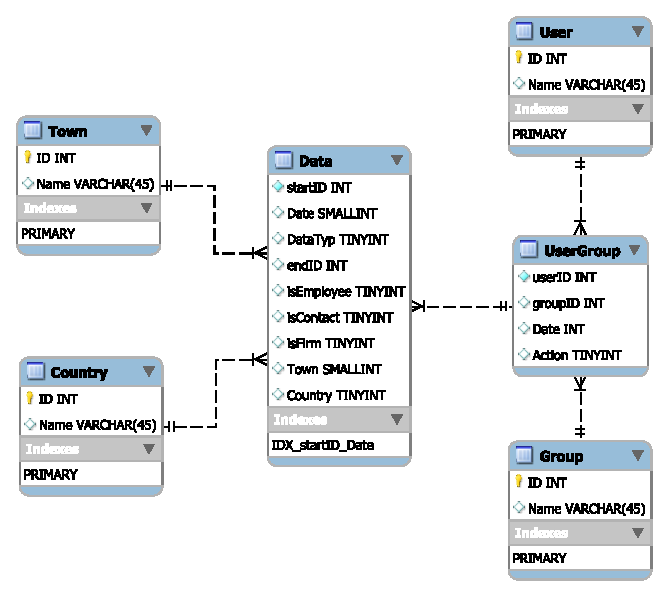
\includegraphics[width=0.8\textwidth, width=0.8\textwidth]{pics/NewSchema.pdf}
\caption{Neue Datenbankschema}
\label{konzept_SchemaNeu}
\end{figure} 

%% ===========================
\subsection{Idee hinter der Data Tabelle}
%% ===========================

Die Idee ist das wenn nur die Informationen zur Lösung des Szenarios abgelegt werden, ist eine Tabelle ausreichend. Diese Tabelle muss es ermöglichen ausgehend von einem Benutzer, alle Personen zu finden die Objekte(Termine, Dokumente usw.) mit Ihm teilen. Dafür sind 3 Spalten ausreichend. Die startID die die Person darstellt von der die Suche ausgeht, DataTyp die aussagt ob es sich in der Tupel um einen Termin oder was anderes handelt und die endID die die person angibt die das Objekt mit der ausgangsperson verbindet. Die anderen Spalten wie z.B. Date dienen lediglich der Filterung des Ergebnisses.

%% ===========================
\subsection{Wörterbücher}
%% ===========================

Um mit den geringeren Speicherkapazitäten die uns zur Verfügung stehen zurechtzukommen sollte auf das Problem der Datenredundanz eingegangen werden. Durch Normalisierung lässt sich Datenredundanz zwar nicht verringern allerdings kann man sie in kontrollierbare Bahnen lenken. Im neuen Schema wurden solche Maßnahmen auf die Spalte Town und Country angewendet. Beide Spalten werden vorraussichtlich Millionen von Werten beinhaltet. Es gibt jedoch nur 193 Länder auf der Welt. Das bedeutet das Wort Deutschland würde sich unzählige mal wiederholen. Die Spalte Country ist vom Datentyp Varchar welches pro Zeichen 2 Byte benötigt. Das wären beim Wort Deutschland 22 Byte. Legt man nun für die Spalte Country eine neue Tabelle an wird in dieser jedes Land nur einmal vermerkt. Jedes Land bekommt einen Schlüssel in Form einer Zahl. In der eigentlichen Tabelle Data werden jetzt nur noch die Zahlen anstatt des vollständig ausgeschrieben Wortes verwendet. Das würde im Fall Deutschland bedeuten das nur noch 1 Byte zur Repräsentation des Wortes benötigt werden. Der Wert 1 Byte kommt Zustande weil TINYINT anstatt INT verwendet wurde. Dies stellt eine weitere Design Entscheidung dar. In der Data Tabelle die alle primären Daten beinhalten wird, wird für jede Spalte der Integer Typ verwendet der eine ausreichend große Menge an zahlen darstellen kann. TINYINT mit 256 Möglichen Werten reicht aus um alle Länder darzustellen sowie die Is-Spalten, die nur 0 oder 1 beinhalten. Die Tabellen Town, Country, User und Group können als eine Art Wörterbuch angesehen werden. Eine weitere Überlegung stellt die Art der des Zugriffes dar. Um die Ergebnismenge um eine bestimmte Stadt zu filtern könnte ein Join der Data Tabelle mit der Town Tabelle durchgeführt werden, was sehr inperformant wäre. Ein effizienterer Ansatz ist erst eine Abfrage auf die Tabelle Town durchzuführen um die ID herauszubekommen. Diesen Wert dann wiederum in der eigentlichen Abfrage an Tabelle Data in der Where Klausel zu verwenden. Dieses Vorgehen kann für die Stadt, das Land und die Gruppenzugehörigkeit angewandt werden.

Die Tabelle GroupDate unterscheidet sich etwas von den anderen Wörterbüchern den dort sind noch weitere Details vermerkt. Diese ermöglichen es Die Zusammenstellung von Gruppen über die Zeit nachzuvollziehen. Action legt fest ob die Tupel einen Eintritt einer Person oder einen Austritt darstellt. Die Spalte Date beinhaltet das Datum des Ereignisses. 

%% ===========================
\subsection{Auswahl geeigneter Zugriffsstrukturen}
%% ===========================

Indizes dienen der Beschleunigung der Suche nach bestimmten Spaltenwerten. Ohne Indexe müsste die H2-Datenbank beim ersten Datensatz beginnen und dann die gesamte Tabelle durchgehen um eine Abfrage zu beantworten. Je größer die Tabelle ist, desto höher sind die Kosten dafür. Daher bietet der Einsatz sich gerade in Anbetracht nach der Forderung von Performance an. Für den Einsatz zur Indexierung von den Tabellen Town, Country, User und Group eignen sich Hash-Indizes. Sie bieten einen extrem schnellen Zugriff auf die Daten. Diese Schnelligkeit ergibt sich aus der Verwendung von Berechnungsvorschriften zur Ermittlung der Position des gesuchten Wertes. Dadurch können Datensätze mit einem einzigen Zugriff gelesen werden. Die Nutzung von Hash-Indizes bringt allerdings Limitierungen mit sich. Eine der wichtigsten ist das Sie nur für Vergleiche("=") verwendet werden können. Somit werden keine Wertebereich-Abfragen("<" oder ">") unterstützt. Es gibt noch andere Nachteile die in \cite{SWB-352401869} nachlesbar sind. 
Für die Tabelle UserGroup eignet sich der Standard Index von H2 der ein B\textsuperscript{+}-Baum verwendet. Dieser kann für die Spalte userID verwendet werden, der den ersten Wert einer Suche darstellt. Der B\textsuperscript{+}-Baum eignet sich auch für die Data-Tabelle. Hier ist der Einsatz eines Mehr-Attribut-Indexes sinnvoll. Der Vorteil eines Mehr-Attribut-Indexes ist, dass bei einer Punkt-Abfrage über alle Zugriffsattributwerte nur ein Indexzugriff erfolgen muss. Indexiert werden in unserem Fall die Spalte startID und Date. Beide Spalten sind sortiert somit bietet sich  die Verwendung eines geclusterten Index an. Geclusterte Indizes sind in der gleichen Form sortiert wie die interne Relation. Ein geclusterter Index unterstützt Bereichsanfragen sehr gut, was bei der Beschränkung auf Zeitspannen von Vorteil sein dürfte.       


%% ===========================
\section{Extract Transform Load Prozess}
%% ===========================

Daten der operativen Systeme unterstützen die wertschöpfende Geschäftsprozesse innerhalb eines Unternehmens. Sie sind demnach auf die Steuerung und Überwachung des Tagesgeschäftes ausgerichtet und daher transaktionsbezogen. Somit sind die Daten in Ihren Begrifflichkeiten häufig nicht vergleichbar und ihrer Bewertung sowie Konsolidierung unterschiedlich. Um die Daten dennoch für analytische Zwecke einzusetzen ist eine Überführung in eine geeigneter Struktur von Vorteil. Eine solche Überführung wird in der Literatur als Extract, Transform, Load (ETL)-Prozess bezeichnet \cite{ElSappagh201191}. 

%% ===========================
\subsection{Extract}
%% ===========================

Zunächst dient die Extraktion der Daten aus dem MSSQL Server der Beschaffung. Überdies können durch den Prozess Daten bereits reduziert,  zusammengeführt und ersetzt werden. Zur korrekten Ermittlung der Analyseergebnisse müssen Sonderfälle in die Ermittlung der Daten beachtet werden. Eine vollständige und korrekte Datenmenge stellt die Grundlage jeder guten Analyse dar.

Die erste Besonderheit die beachtet werden sollte das die Analyse den Faktor Zeit beachtet. Bei Analysen über die Zeit ist zu beachten das Daten sich im Laufe der Zeit verändern und dies berücksichtigt werden muss. Die Tabelle Changelogbook bietet uns die Möglichkeit Veränderungen in den Datensätzen zu ermitteln. Eine der zu beachtenden Veränderungen über die Zeit ist die Gruppenkonstellation, da Personen Gruppen verlassen oder beitreten können. Datensätze können sich nicht nur über die Zeit verändern sondern können sich auch über diese erstrecken. Termine wie Tagungen und der gleichen erstrecken sich über mehrere Tage. In der MSSQL Datenbank werden die Termin als ein Datensatz beachtet. Wenn ein Termin über mehrere Tage geht sollte in der Gewichtung stärker gewertet werden als ein Termin über einen Tag. Deswegen sollte im Ergebnis der SQL-Query vermerkt werden das dieser Termin mehrere Tage ging damit das in der Transformation berücksichtigt werden kann. 

Eine weitere Besonderheit ergibt sich durch das Nutzungsverhalten der Benutzer, die damit die Einträge der Datenbank verfälschen. CAS genesisWorld ermöglicht es Termine zu schieben. Diese Funktion wird von manchen Nutzern missbraucht. Anstatt für einen ähnlichen Termin einen neuen Eintrag anzulegen wird ein alter aus Bequemlichkeit geschoben. Das hat zur Folge das Termine die statt gefunden haben in der Datenbank nicht mehr existieren. Um trotzdem diese Termine zu berücksichtigen wurde sich folgendes Überlegt. Dem Changelogbook lässt sich entnehmen ob das Feld start\_dt und end\_dt verändert wurden. Um sagen zu können das der Termin stattgefunden und nur geschoben wurde müssen zwei Sachen überprüft werden. Zuerst ob der Termin vor dem angegeben Zeitpunkt geschoben wurde. Falls ja kann dies als reguläre Schiebung angesehen werden. Falls danach wird noch überprüft ob der neu Zeitpunkt in der Zukunft liegt und der Operation.Typ ein Update war. 

Zur Zwischenspeicherung der Daten wird das CSV Dateiformat eingesetzt. Dieser Zwischenschritt dient der Nachvollziehbarkeit zwischen der Beschaffung der Daten und deren Transformation. Bei der Fehlersuche beispielsweise kann dies sehr hilfreich sein.  

%% ===========================
\subsection{Transform}
%% ===========================

Zu Beginn der Transformation werden Filterungen durchgeführt. Unter der Filterung von operativen Daten, versteht man eine Bereinigung syntaktischer oder inhaltlicher Defekte der zu übernehmenden Daten. Die MSSQL Datenbank besteht zu 37\% aus Null Werten und zu 4\% aus Leeren Feldern. Daten die beispielsweise null Werte enthalten die für die Ermittlung des Datums benötigt werden sind für die Analyse nicht zu gebrauchen. Sie können daher im laufe des Prozesses aus den Daten entfernt werden. Bei den anderen Filteroperationen können Nullwerte jedoch vernachlässigt werden da sie nicht unbedingt benötigt werden und nur ein zusätzliches Feature Darstellen.

Der nächste Schritt wäre die Harmonisierung der Daten. Unter anderem besitzen die Telefonnummern kein einheitliches Format. Sie wurde manuell von Sachbearbeitern eingetragen. Das erfordert ein Zusammenführen aller Nummern in ein einheitliches Format welches einen automatischen Vergleich ermöglicht.

Die in der Extraktion genannten Besonderheiten müssen durch unterschiedliche Query-Abfragen besorgt werden. Dadurch ist zum Abschluss der Transformation eine Zusammenführung der Daten notwendig. Das Ergebnis wird anschließend in einer CSV-Datei abgelegt. 

%% ===========================
\subsection{Load}
%% ===========================

Beim Laden der Datensätze in den H2 kommt ein sogenannter \"bulk load\" Prozess zum Einsatz. Dieser wird häufig beim laden von großen Datenmengen aus einer Datei eingesetzt. Er ermöglicht ein wesentlich schnelleres Befüllen der Datenbank bei großen Datenmengen im Gegensatz zu den INSERT-Operationen.

%% ===========================
\section{Sicherstellung der Aktualität der Daten}
%% ===========================

Systeme die auf den Datenbestand anderer Systeme aufbauen können zwei verschiedenen Ansätze zur Sicherstellung ihrer Aktualität verfolgen. Unser nebenläufiges System bezeichnen wir als A und das System das den original Datenbestand darstellt als B. Einer der Ansätze ist die Intervall basierende Nachfrage über Veränderungen von A. Hierbei fragt A bei B in festgelegten Intervallen nach ob Daten verändert wurden. Die Wahl des Nachfrage-Intervalls stellt dabei eine der größten Schwierigkeiten dar. Ist der Intervall zu groß, sinkt die Aktualität des Datenbestandes. Ist er zu klein entsteht bei B ein starke Belastung. Der andere Ansatz ist das B Benachrichtigungen an A über Veränderungen sendet. Dadurch werden keine unnötigen Abläufe angestoßen, da nur im Falle von neuen Daten Prozesse in Bewegung gesetzt werden. Zwar wird die Aktualität der Daten gewährleistet jedoch büßt A an Entscheidungsfreiheit ein. A kann nicht mehr selbst entscheiden wann aktualisiert werden soll. Der zweite Ansatz ist zwar effizienter jedoch nicht immer umsetzbar. Das kann Technische Gründe oder unternehmenspolitische Gründe haben, die eine Veränderung des Legacy Systems ausschließen.  

\begin{figure}[htbp]
\centering
  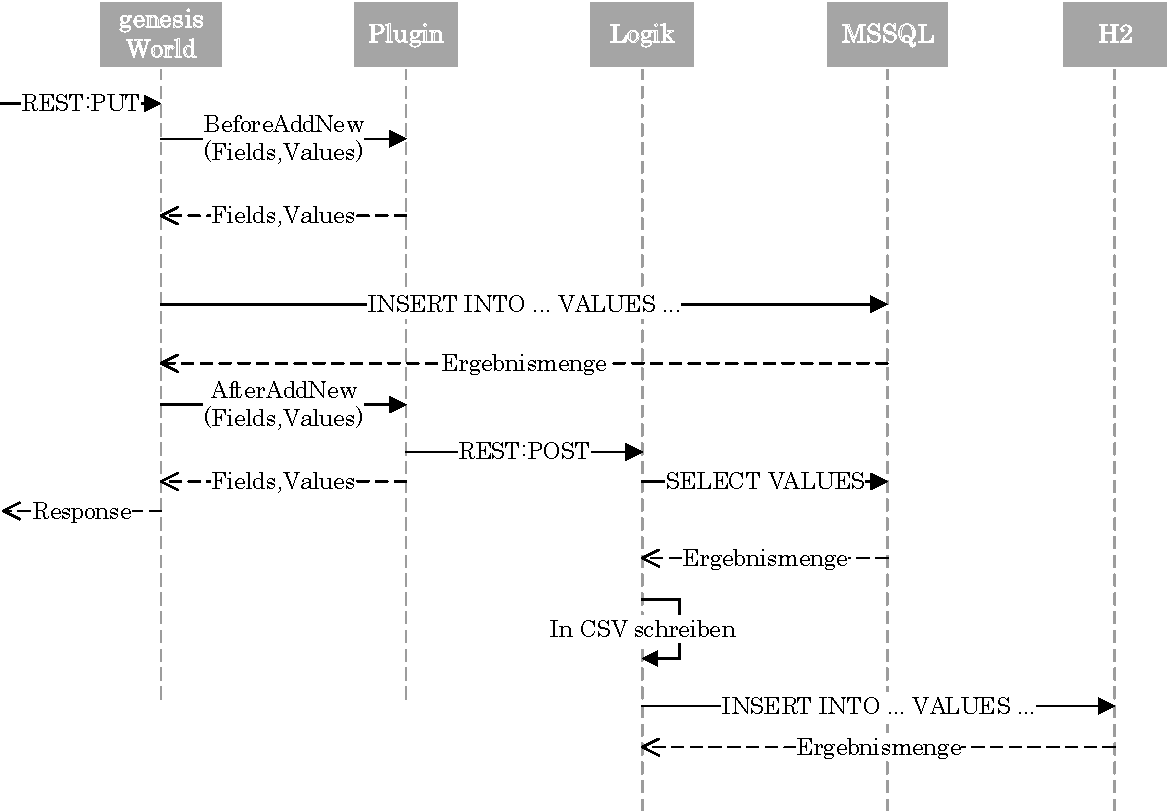
\includegraphics[width=1.0\textwidth, width=1.0\textwidth]{pics/sequenzdiagramm.pdf}
\caption{Sequenzdiagramm eines Updates}
\label{konzept_sequenz}
\end{figure}

In CAS genesisWorld gibt es eine Möglichkeit den zweiten Ansatz umzusetzen. Die Idee dabei ist den Applikationsserver um ein sogenanntes Plugin zu erweitern das über Veränderungen in der MSSQL Datenbank benachrichtigt wird. Realisiert wird ein solches Plugin als COM-Objekt welches das Interface IGWSDKDataPlugIn implementiert. Das erstellte COM-Objekt wird im Server von CAS genesisWorld registriert. Der Server delegiert, wie in Abbildung \ref{konzept_sequenz} zu sehen, bei einer Datenoperation den Aufruf an die für den jeweiligen Datensatz-Typen registrierten PlugIns. Das Plugin selbst besitzt einen REST-Client der einen POST an die Logik sendet. Sie enthält die GGUID des Veränderten Datensatzes. Mithilfe dessen die Extraktion des betroffenen Datensatzes durchgeführt wird. Der neue/veränderte Datensatz wird zuerst in einer CSV zwischengespeichert und anschließend an die H2-Datenbank gesendet.

%% ===========================
\section{Darstellungskonzepte}
%% ===========================

Bei der Konzeption einer Darstellung ist die Grad der Granularität von Informationen ein wichtiger Leitfaktor zur Bestimmung des Aufbaus. In unserem Fall ist nicht die Eigenschaft einer Verbindung von interessiere sondern ihr Typ und ihre Häufigkeit zu einer bestimmten Person. Da keine Detailinformationen zur Verbindung vorhanden sind kann jeder Benutzer frei wählen von welcher Person ausgehend die Analyse stattfinden soll. Für die Oberfläche bedeutet dies einen Einstiegspunkt in Form eines Fensters in dem der jeweilige Benutzername von dem die Suche ausgehen soll, eingegeben wird.

Nach dem Login findet eine Weiterleitung auf die eigentliche Seite statt. Dessen Aufbau ist in Abbildung \ref{konzept_darstellung} (a) zu sehen. Oben auf der Seite sind alle Regler, CheckBoxen und Eingabefelder zur Filterung der Ergebnismenge zu finden. Direkt darunter befindet sich das Diagramm das die Ergebnismenge einer Abfrage darstellt.

Diagrammtypen gibt es viele jedoch ergeben sich Einschränkungen durch das Framework welches zu Realisierung verwendet wird. Im Prinzip lässt sich jede Darstellung verwirklichen allerdings ist das Aufwand Nutzen Verhältnis zu berücksichtigen. In einer Vorauswahl wurden einige Typen ausgewählt die in Abbildung \ref{konzept_darstellung} (b)-(f) dargestellt sind. 

Netzdiagramme geben Eigenschaften verschiedener Systeme wieder. Sie eignen sich daher gut zur Darstellung von Ausprägungen. Für unsere Form der Daten ist diese Darstellung gänzlich ungeeignet. Mithilfe von Liniendiagrammen lassen sich Trends und Zeitreihen darstellen. Die Verwendung verschiedener Linien ermöglicht zudem die Darstellung mehrerer Trends. Die Benutzung dieses Diagramms macht keinen Sinn da die Ergebnismenge sich nicht auf verschiedene Zeitpunkte bezieht sondern die Summe der Werte in der Zeitreihe beinhaltet. Eine Tree Map dient der Abbildung von hierarchischen Daten. Dabei steht jede Fläche eines Rechtecks im proportionalen Zusammenhang zur Gesamtfläche. Die Beachtung von Größenverhältnissen stellt einen nützliche Eigenschaft für unsere Daten dar. Eine Hierarchie innerhalb der Daten ist nicht im klassischen Sinn vorhanden. Vielmehr würde jedes Rechteck aus dem jeweiligen Anteilen der Verbindungstypen bestehen. Beispielweise könnte die Person Ludwig Neer wiederum in Rechtecke unterteilt werden, die die Anzahl der E-Mails, Termine usw. enthalten. Das würde allerdings schnell zu einer schlechten Übersicht führen da viel zu viele Kacheln dargestellt werden müssen. Kreisdiagramme ermöglichen eine Betrachtung der Gesamtheit zu ihren Einzelstücken, da der Kreis ein geschlossenes System darstellt. Allerdings müssen alle Teile sich auf die gleiche Basis beziehen. Es eignet sich hervorragend zur Darstellung von Verhältnissen. Möchte man jedoch noch die Zusammenstellung eines einzelnen Stückes noch einmal aufteilen ist ein zweite Ansicht nötig. Am besten dürfte sich ein Balkendiagramm eignen. Reihenfolgen beispielsweise lasse sich durch die resultierenden Stufen sehr gut darstellen. Balken selbst lassen sich außerdem in einzelne Teile aufspalten ohne die Übersichtlichkeit zu verringern. Gegenüber dem Kreisdiagramm kann es zwar keine Betrachtung des Gesamten liefern allerdings ist das in diesem Anwendungsfall auch nicht nötig. 

\begin{figure}[htbp]
\subfigure[Grober Entwurf des Aufbaus der Hauptseite]{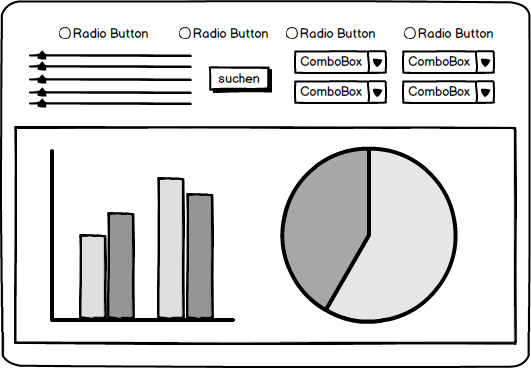
\includegraphics[width=0.49\textwidth]{pics/konzept_mockup.png}}\hfill
\subfigure[Tortendiagramm]{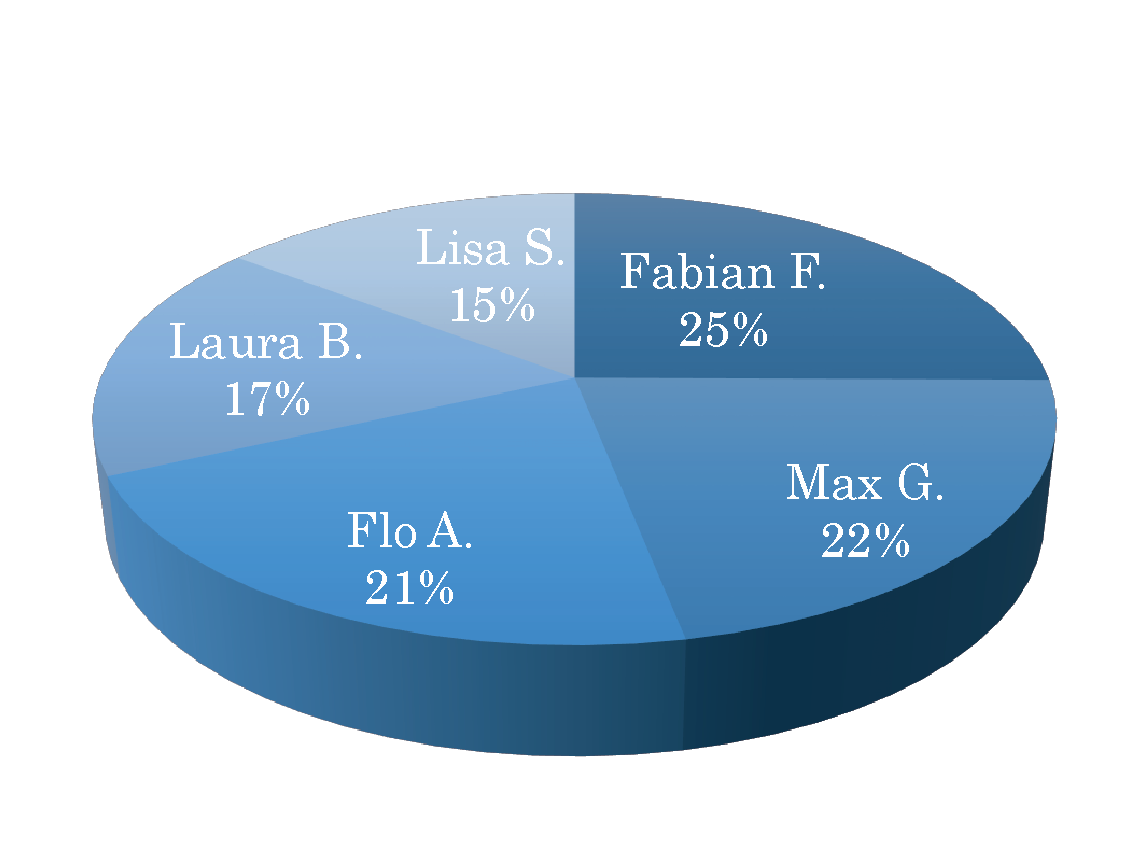
\includegraphics[width=0.49\textwidth]{pics/konzept_tortendiagramm.pdf}}\hfill
\subfigure[Balkendiagramm]{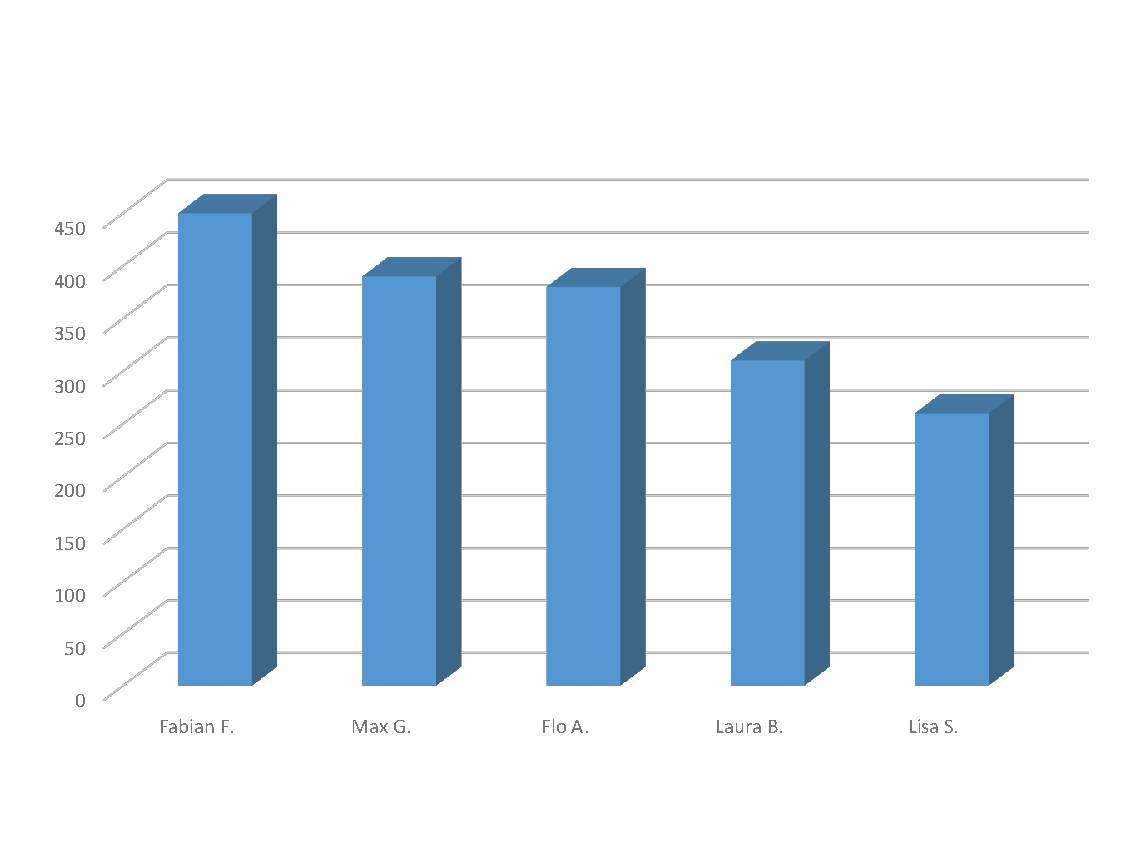
\includegraphics[width=0.49\textwidth]{pics/konzept_balkendiagramm.pdf}}\hfill
\subfigure[Tree Map]{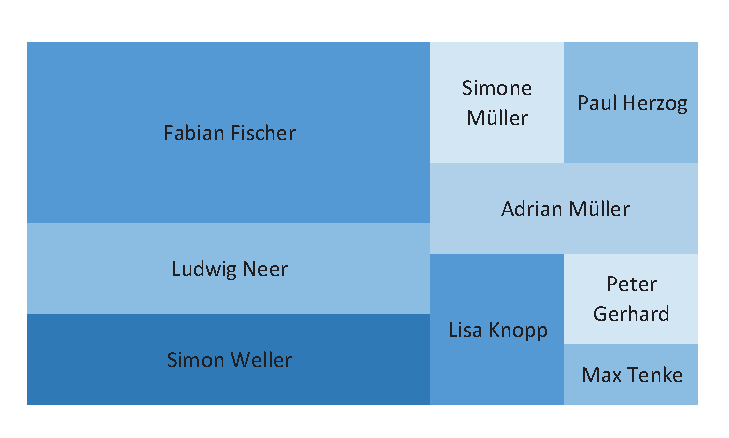
\includegraphics[width=0.49\textwidth]{pics/konzept_tree_map.pdf}}\hfill
\subfigure[Liniendiagramm]{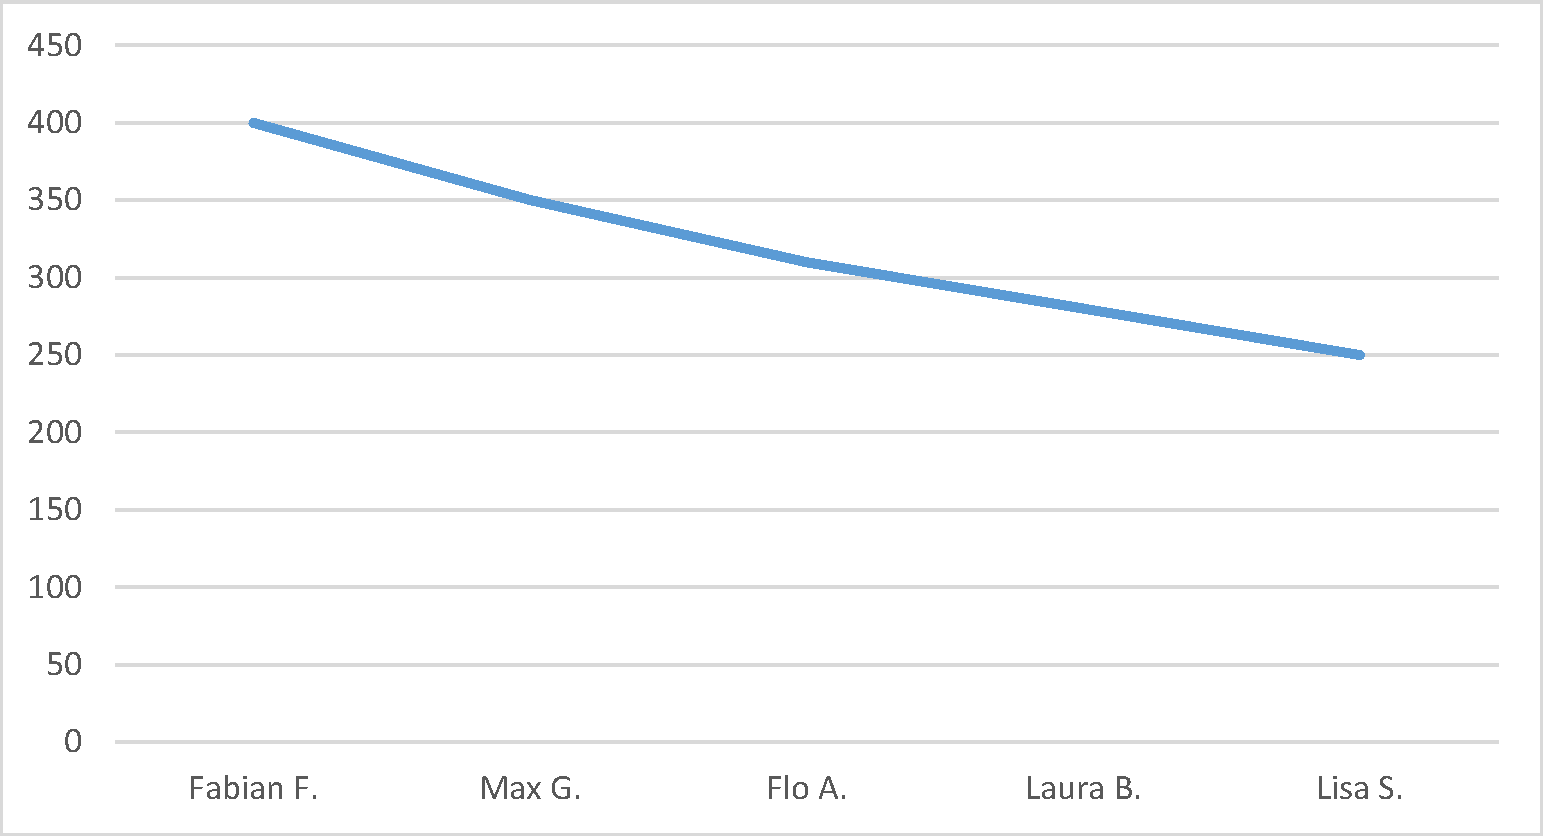
\includegraphics[width=0.49\textwidth]{pics/konzept_liniendiagramm.pdf}}\hfill
\subfigure[Netzdiagramm]{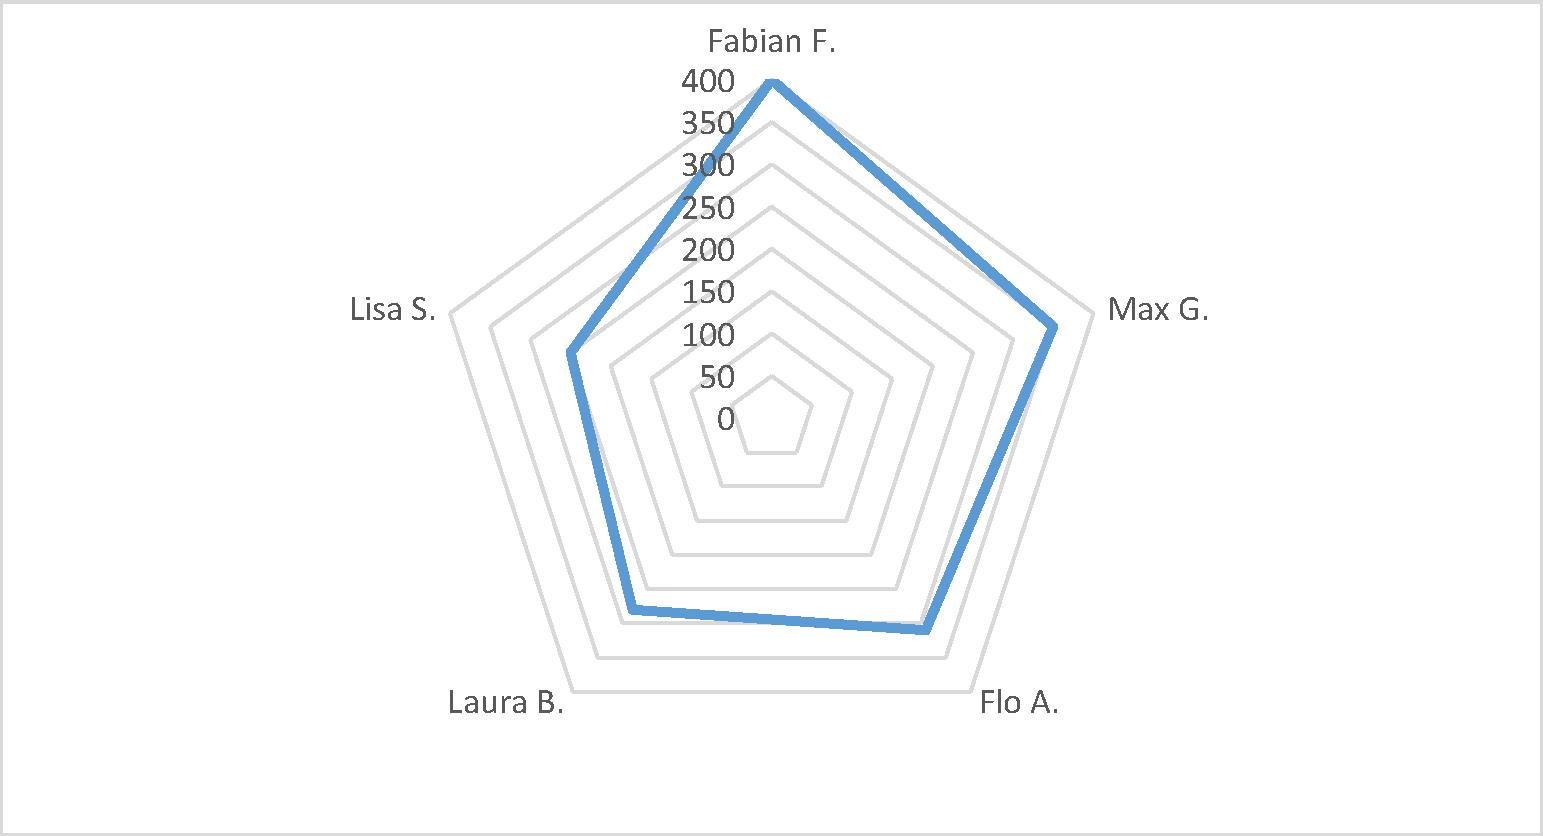
\includegraphics[width=0.49\textwidth]{pics/konzept_netzdiagramm.pdf}}
\caption{Entwürfe der Oberfläche}
\label{konzept_darstellung}
\end{figure}